\documentclass[Nike]{tuberlinbeamer}
\usepackage[english]{babel}  % 'babel' muss geladen werden
\usepackage[utf8]{inputenc}  % optional, aber empfehlenswert
\usepackage[T1]{fontenc}
\usepackage{
	tikz,
	pgfplots,
	xparse,
	boxedminipage2e,
	amsmath,
	hyperref
	}
\usepackage[style=verbose,backend=biber]{biblatex}
%\bibliographystyle{JHEP}
\bibliography{other/references.bib}
%\addbibresource{other/references}
\usepackage[font={small}]{caption}
\usetikzlibrary{
	shapes,
	arrows,
	snakes,
	chains}
\tikzstyle{arrow} = [thick,->,>=stealth]

% Die ueblichen Angaben
\title{Model Order Reduction of Rarefied Gases Using Neural Networks}
\subtitle{}
\author[Zachary Schellin]{Zachary Schellin}
\institute{Institut f\"ur Numerische Fluiddynamik}

% Eigenes Logo einfuegen:
\renewcommand{\pathtomylogo}{csm_cfd_logo_invers_ohne_schrift_blauer_hintergrund_3fa262aacf.png}
\AtBeginSection[]
{
	\begin{frame}
		\frametitle{Table of Contents}
		\tableofcontents[currentsection]
	\end{frame}
}
\begin{document}

\begin{frame}
\maketitle
\end{frame}


\begin{frame}[fragile]{Outline}
\tableofcontents
\end{frame}
\section{Introduction}
%%%%%%%%%%%%%%%%%%%%%%%%%%%%%%%%%%%%%%%%%%%%%%%%%%%%%%%%%%%%%%%%%%%%%%%%
\section{The BGK-Model}
\begin{frame}[fragile]{Governing equations}
	\begin{itemize}
		\item The Boltzmann equation approximated by $\boldsymbol{Q}$ the BGK operator as a source term with
		\begin{equation}
		\partial_t f + v \partial_x f = \overbrace{\frac{1}{\tau} (M_f - f)}^{Q}
		\end{equation}

		\item The equilibrium solution is a Maxwellian distribution $\boldsymbol{M_f}$ with
		\begin{equation}
		M_f = \frac{\rho(x,t)}{(2\pi R T(x,t))^{\frac{3}{2}}}\exp(-\frac{(v - u(x,t))^2}{2 R T(x,t)}) 
		\end{equation}

		\item The duration to evolve into equilibrium is given by the relaxation time $\boldsymbol{\tau}$ with
		\begin{equation}
		\tau^{-1} = \frac{\rho(x,t)T^{1-\nu}(x,t)}{Kn}
		\end{equation}

		\item The rarefaction level is defined over the Knudsen number $\boldsymbol{Kn}$ with
		\begin{equation}
		Kn = \frac{\lambda}{l}
		\end{equation}
	\end{itemize}
	\footfullcite{PhysRev.94.511}
\end{frame}

\begin{frame}[fragile]{Knudsen number}
	\begin{itemize}
		\item Solution is $f(x,v,t)$ in 1D and $f(x,y,v_x,v_y,t)$ in 2D and $f(x,y,z,v_x,v_y,v_z,t)$ in 3D 
	\end{itemize}
	\hfill
	\begin{center}
			\begin{figure}
			\centering
			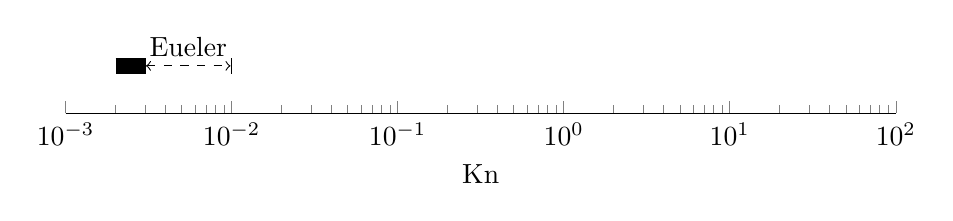
\begin{tikzpicture}
\begin{axis}[
    y=3cm,            % y unit vector
    hide y axis,        % hide the y axis
    xmode = log,        % logarithmic x axis
    axis x line*=bottom,% only show the bottom x axis line, without an arrow tip
    xmin=1e-3, xmax=1e2,% range for the x axis
    xlabel = Kn,
    width=\textwidth,
]
\addplot [no markers, line width=6pt] table {%
0.002 1
0.003 1
};
\draw [|<->|,dashed] (axis cs:0.003,1) -- (axis cs: 0.01,1) node[midway,above] {Eueler};
\end{axis}
%\begin{scope}[decoration=brace]
%	\draw [decorate] (current axis.south-|0.003) -- (current axis.south-|0.01) node[midway,above] {Eueler};
%\end{scope}
%\draw [] (axis cs:0.25,2.1) node[above] {\(T\)};
%\begin{scope}[decoration=brace]
%\pgfdecorationsegmentamplitude=5pt
%\draw[decorate] (T2.south east) -- (T0.south west) node[midway,below=\pgfdecorationsegmentamplitude] {Part 1};
%\draw[decorate] (T14.south east) -- (T3.south west) node[midway,below=\pgfdecorationsegmentamplitude] {Part 2};
%\draw[decorate] (T20.south east) -- (T15.south west) node[midway,below=\pgfdecorationsegmentamplitude] {Part 3};
%\end{scope}
\end{tikzpicture}
			\caption{Partitioning of $Kn$, the Knudsen number, into levels of rarefaction.}
			\label{Fig:ExpKN}
			\footfullcite{NumaKUL}
		\end{figure}
	\end{center}
\end{frame}

\begin{frame}[fragile]{Discretization in space and velocity space in 1D}
	\begin{itemize}
		\item Space and time discretization considering a uniform grid i.e.\\ $x_j = j\Delta x$ and $j\in \mathbb{Z}$, $v_k = k\Delta v$ and $k\in \mathbb{Z}$, $t^i=i\Delta t$ and $t\in \mathbb{N}$,
		\item is leading from the full PDE to a set of ODE's in time 
			\begin{equation}
			\partial_t f_{j,k} = -(v_k)_1D_x f|_{j,k}(t) + \frac{1}{\tau}({M_f}_{j,k}(t) - f_{j,k}(t))\mathrm{.}
			\end{equation}
		\item $KJ$ first-order differential equations need to be evaluated when $K$ and $J$ are the number of gridpoints in space and velocity space.
		\item In 3D there are $K^3J^3$ first-order differential equations.
		\item The discretization in velocity space requires the computation of the moments of $f$.
	\end{itemize}
\end{frame}

\begin{frame}[fragile]{Moments/ Expected values of $f$}
	\begin{itemize}
		\item By multiplying the collision invariants $\Phi(v)=[1,v,\frac{1}{2}v^2]$ with $f$ and integrating in velocity space $v$ the moments are obtained.
		\item The first moment/ the Density is
		\begin{equation}
				\rho(x,t) = \int\! f \,\mathrm{d}v \,,
		\end{equation}
		\item the second moment/ the Momentum is
		\begin{equation}
			\rho(x,t) u(x,t) = \int\! v f \,\mathrm{d}v \,,
		\end{equation}
		\item the third moment/ the kinetic Energy is
		\begin{equation}
			E(x,t) = \int\! \frac{1}{2}v^2 f  \,\mathrm{d}v \,.
		\end{equation}
	\end{itemize}
\end{frame}

\begin{frame}[fragile]{Moments/ Expected values of $f$}
	\begin{center}
		\begin{figure}
			% This file was created by tikzplotlib v0.9.6.
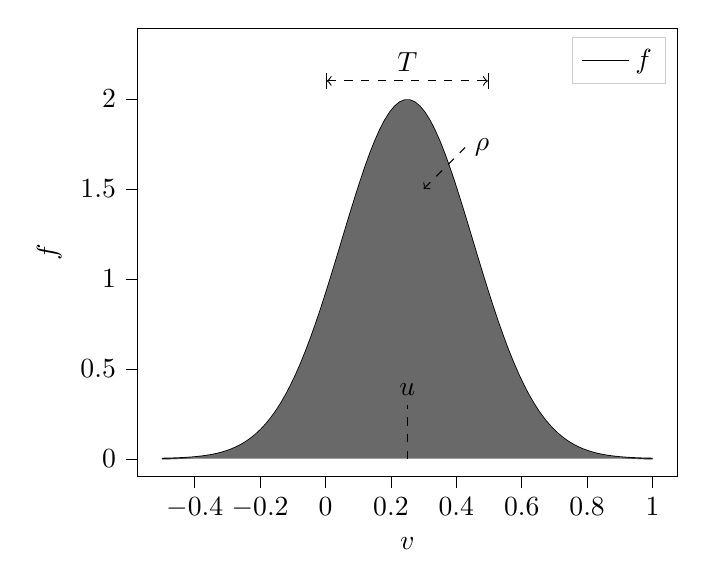
\begin{tikzpicture}

\begin{axis}[
legend cell align={left},
legend style={fill opacity=0.8, draw opacity=1, text opacity=1, draw=white!80!black},
tick align=outside,
tick pos=left,
x grid style={white!69.0196078431373!black},
xlabel={\(v\)},
xmin=-0.575, xmax=1.075,
xtick style={color=black},
y grid style={white!69.0196078431373!black},
ylabel={\(f\)},
ymin=-0.0978129180007683, ymax=2.39285680307655,
ytick style={color=black}
]

\addplot [semithick, black]
table {%
	-0.5 0.00176297841183723
	-0.484848484848485 0.00233549990938288
	-0.46969696969697 0.00307623995021814
	-0.454545454545455 0.0040287289903483
	-0.439393939393939 0.00524594088238899
	-0.424242424242424 0.00679182087082491
	-0.409090909090909 0.00874292085377632
	-0.393939393939394 0.0111901101946249
	-0.378787878787879 0.0142403174963827
	-0.363636363636364 0.018018244420721
	-0.348484848484849 0.0226679772544878
	-0.333333333333333 0.0283544060972295
	-0.318181818181818 0.0352643460570684
	-0.303030303030303 0.0436072406856785
	-0.287878787878788 0.0536153162176469
	-0.272727272727273 0.0655430473059348
	-0.257575757575758 0.0796657922473926
	-0.242424242424242 0.0962774595613305
	-0.227272727272727 0.115687079522804
	-0.212121212121212 0.138214174964358
	-0.196969696969697 0.164182856129127
	-0.181818181818182 0.193914604924168
	-0.166666666666667 0.227719764364528
	-0.151515151515151 0.265887808434693
	-0.136363636363636 0.308676534413689
	-0.121212121212121 0.356300391543538
	-0.106060606060606 0.408918233661475
	-0.0909090909090909 0.466620855301653
	-0.0757575757575757 0.529418736525693
	-0.0606060606060606 0.597230476778283
	-0.0454545454545454 0.669872437749538
	-0.0303030303030303 0.747050135179608
	-0.0151515151515151 0.828351915965591
	0 0.91324542694511
	0.0151515151515151 1.00107732368077
	0.0303030303030303 1.09107658129022
	0.0454545454545454 1.18236165636822
	0.0606060606060607 1.2739516126026
	0.0757575757575758 1.36478116780159
	0.0909090909090909 1.45371945330681
	0.106060606060606 1.53959210603912
	0.121212121212121 1.62120614747867
	0.136363636363636 1.69737695187443
	0.151515151515151 1.76695647690227
	0.166666666666667 1.82886183207001
	0.181818181818182 1.88210320029322
	0.196969696969697 1.92581011126961
	0.212121212121212 1.95925509432898
	0.227272727272727 1.98187381354832
	0.242424242424242 1.99328090666395
	0.257575757575758 1.99328090666395
	0.272727272727273 1.98187381354832
	0.287878787878788 1.95925509432898
	0.303030303030303 1.92581011126961
	0.318181818181818 1.88210320029322
	0.333333333333333 1.82886183207001
	0.348484848484849 1.76695647690227
	0.363636363636364 1.69737695187443
	0.378787878787879 1.62120614747867
	0.393939393939394 1.53959210603912
	0.409090909090909 1.45371945330681
	0.424242424242424 1.36478116780159
	0.439393939393939 1.2739516126026
	0.454545454545455 1.18236165636822
	0.46969696969697 1.09107658129022
	0.484848484848485 1.00107732368077
	0.5 0.91324542694511
	0.515151515151515 0.828351915965591
	0.53030303030303 0.747050135179608
	0.545454545454545 0.669872437749538
	0.560606060606061 0.597230476778283
	0.575757575757576 0.529418736525694
	0.590909090909091 0.466620855301653
	0.606060606060606 0.408918233661474
	0.621212121212121 0.356300391543538
	0.636363636363636 0.308676534413689
	0.651515151515152 0.265887808434693
	0.666666666666667 0.227719764364528
	0.681818181818182 0.193914604924168
	0.696969696969697 0.164182856129127
	0.712121212121212 0.138214174964358
	0.727272727272727 0.115687079522804
	0.742424242424242 0.0962774595613305
	0.757575757575758 0.0796657922473926
	0.772727272727273 0.0655430473059348
	0.787878787878788 0.0536153162176469
	0.803030303030303 0.0436072406856785
	0.818181818181818 0.0352643460570684
	0.833333333333333 0.0283544060972294
	0.848484848484849 0.0226679772544878
	0.863636363636364 0.018018244420721
	0.878787878787879 0.0142403174963826
	0.893939393939394 0.0111901101946249
	0.909090909090909 0.00874292085377631
	0.924242424242424 0.00679182087082491
	0.939393939393939 0.00524594088238899
	0.954545454545455 0.0040287289903483
	0.96969696969697 0.00307623995021814
	0.984848484848485 0.00233549990938288
	1 0.00176297841183723
};
\addlegendentry{\(f\)}

\path [draw=none, fill=white!41.1764705882353!black]
(axis cs:-0.5,0.00176297841183723)
--(axis cs:-0.484848484848485,0.00233549990938288)
--(axis cs:-0.46969696969697,0.00307623995021814)
--(axis cs:-0.454545454545455,0.0040287289903483)
--(axis cs:-0.439393939393939,0.00524594088238899)
--(axis cs:-0.424242424242424,0.00679182087082491)
--(axis cs:-0.409090909090909,0.00874292085377632)
--(axis cs:-0.393939393939394,0.0111901101946249)
--(axis cs:-0.378787878787879,0.0142403174963827)
--(axis cs:-0.363636363636364,0.018018244420721)
--(axis cs:-0.348484848484849,0.0226679772544878)
--(axis cs:-0.333333333333333,0.0283544060972295)
--(axis cs:-0.318181818181818,0.0352643460570684)
--(axis cs:-0.303030303030303,0.0436072406856785)
--(axis cs:-0.287878787878788,0.0536153162176469)
--(axis cs:-0.272727272727273,0.0655430473059348)
--(axis cs:-0.257575757575758,0.0796657922473926)
--(axis cs:-0.242424242424242,0.0962774595613305)
--(axis cs:-0.227272727272727,0.115687079522804)
--(axis cs:-0.212121212121212,0.138214174964358)
--(axis cs:-0.196969696969697,0.164182856129127)
--(axis cs:-0.181818181818182,0.193914604924168)
--(axis cs:-0.166666666666667,0.227719764364528)
--(axis cs:-0.151515151515151,0.265887808434693)
--(axis cs:-0.136363636363636,0.308676534413689)
--(axis cs:-0.121212121212121,0.356300391543538)
--(axis cs:-0.106060606060606,0.408918233661475)
--(axis cs:-0.0909090909090909,0.466620855301653)
--(axis cs:-0.0757575757575757,0.529418736525693)
--(axis cs:-0.0606060606060606,0.597230476778283)
--(axis cs:-0.0454545454545454,0.669872437749538)
--(axis cs:-0.0303030303030303,0.747050135179608)
--(axis cs:-0.0151515151515151,0.828351915965591)
--(axis cs:0,0.91324542694511)
--(axis cs:0.0151515151515151,1.00107732368077)
--(axis cs:0.0303030303030303,1.09107658129022)
--(axis cs:0.0454545454545454,1.18236165636822)
--(axis cs:0.0606060606060607,1.2739516126026)
--(axis cs:0.0757575757575758,1.36478116780159)
--(axis cs:0.0909090909090909,1.45371945330681)
--(axis cs:0.106060606060606,1.53959210603912)
--(axis cs:0.121212121212121,1.62120614747867)
--(axis cs:0.136363636363636,1.69737695187443)
--(axis cs:0.151515151515151,1.76695647690227)
--(axis cs:0.166666666666667,1.82886183207001)
--(axis cs:0.181818181818182,1.88210320029322)
--(axis cs:0.196969696969697,1.92581011126961)
--(axis cs:0.212121212121212,1.95925509432898)
--(axis cs:0.227272727272727,1.98187381354832)
--(axis cs:0.242424242424242,1.99328090666395)
--(axis cs:0.257575757575758,1.99328090666395)
--(axis cs:0.272727272727273,1.98187381354832)
--(axis cs:0.287878787878788,1.95925509432898)
--(axis cs:0.303030303030303,1.92581011126961)
--(axis cs:0.318181818181818,1.88210320029322)
--(axis cs:0.333333333333333,1.82886183207001)
--(axis cs:0.348484848484849,1.76695647690227)
--(axis cs:0.363636363636364,1.69737695187443)
--(axis cs:0.378787878787879,1.62120614747867)
--(axis cs:0.393939393939394,1.53959210603912)
--(axis cs:0.409090909090909,1.45371945330681)
--(axis cs:0.424242424242424,1.36478116780159)
--(axis cs:0.439393939393939,1.2739516126026)
--(axis cs:0.454545454545455,1.18236165636822)
--(axis cs:0.46969696969697,1.09107658129022)
--(axis cs:0.484848484848485,1.00107732368077)
--(axis cs:0.5,0.91324542694511)
--(axis cs:0.515151515151515,0.828351915965591)
--(axis cs:0.53030303030303,0.747050135179608)
--(axis cs:0.545454545454545,0.669872437749538)
--(axis cs:0.560606060606061,0.597230476778283)
--(axis cs:0.575757575757576,0.529418736525694)
--(axis cs:0.590909090909091,0.466620855301653)
--(axis cs:0.606060606060606,0.408918233661474)
--(axis cs:0.621212121212121,0.356300391543538)
--(axis cs:0.636363636363636,0.308676534413689)
--(axis cs:0.651515151515152,0.265887808434693)
--(axis cs:0.666666666666667,0.227719764364528)
--(axis cs:0.681818181818182,0.193914604924168)
--(axis cs:0.696969696969697,0.164182856129127)
--(axis cs:0.712121212121212,0.138214174964358)
--(axis cs:0.727272727272727,0.115687079522804)
--(axis cs:0.742424242424242,0.0962774595613305)
--(axis cs:0.757575757575758,0.0796657922473926)
--(axis cs:0.772727272727273,0.0655430473059348)
--(axis cs:0.787878787878788,0.0536153162176469)
--(axis cs:0.803030303030303,0.0436072406856785)
--(axis cs:0.818181818181818,0.0352643460570684)
--(axis cs:0.833333333333333,0.0283544060972294)
--(axis cs:0.848484848484849,0.0226679772544878)
--(axis cs:0.863636363636364,0.018018244420721)
--(axis cs:0.878787878787879,0.0142403174963826)
--(axis cs:0.893939393939394,0.0111901101946249)
--(axis cs:0.909090909090909,0.00874292085377631)
--(axis cs:0.924242424242424,0.00679182087082491)
--(axis cs:0.939393939393939,0.00524594088238899)
--(axis cs:0.954545454545455,0.0040287289903483)
--(axis cs:0.96969696969697,0.00307623995021814)
--(axis cs:0.984848484848485,0.00233549990938288)
--(axis cs:1,0.00176297841183723)
--cycle;
\addlegendimage{area legend, draw=none, fill=white!41.1764705882353!black}




\draw [dashed,|<->|] (axis cs:0,2.1) -- (axis cs:0.5,2.1);
\draw [] (axis cs:0.25,2.1) node[above] {\(T\)};
\draw [dashed] (axis cs:0.25,0)--(axis cs:0.25,0.3);
\draw [] (axis cs:0.25,0.3) node[above] {\(u\)};
\draw [dashed,<-] (axis cs:0.3,1.5)-- +(15pt,15pt) node[right] {\(\rho\)};
\end{axis}
\end{tikzpicture}

			\caption{Illustration of the linkage between the macroscopic quantities of the gas flow and the distribution function \(f\).}
		\end{figure}
	\end{center}
\end{frame}
\section{Sod's shock tube}
%%%%%%%%%%%%%%%%%%%%%%%%%%%%%%%%%%%%%%%%%%%%%%%%%%%%%%%%%%%%%%%
\begin{frame}[fragile]{Sod's shock tube}
	\begin{columns}
		\begin{column}{.5\textwidth}
				\begin{figure}
					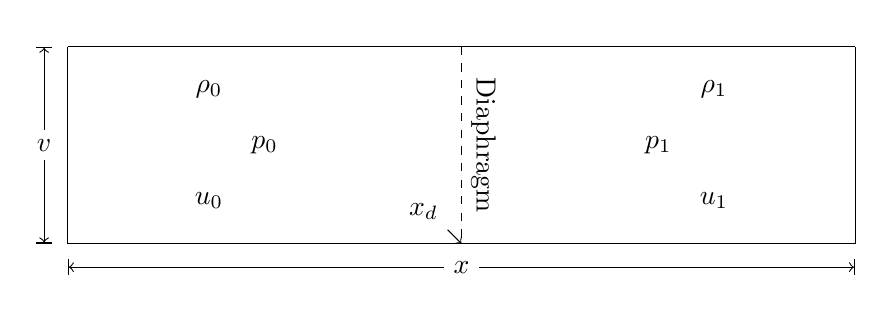
\begin{tikzpicture}
% place nodes
\node[] at (0, 0) (a) {};
\node[] at (0,-.3) (a1){};
\node[] at (-.3,0) (a2){};
\node[] at (10,0) (b) {};
\node[] at (10,-.3) (b1){};

\node[] at (0,2.5)  (c) {};
\node[] at (-.3,2.5) (c1){};
\node[] at (10,2.5) (d) {};

\node[] at (5,2.5)  (e) {};
\node[] at (5,0) (f) {};

% draw edges  
\draw[] (a.center) -- (b.center) {};
\draw[|<->|] (a1.center) -- (b1.center) node[midway,fill=white] (TextNode) {\(x\)};
\draw[] (a.center) -- (c.center) {};
\draw[|<->|] (a2.center) -- (c1.center) node[midway,fill=white] (TextNode) {\(v\)};
\draw[] (c.center) -- (d.center) node[above] {};
\draw[] (d.center) -- (b.center) node[above] {};
\draw[dashed] (e.center) -- (f.center) node[sloped,above,midway] {Diaphragm};
\draw[<-] (f.center)-- +(-5pt,5pt) node[above left] {\(x_d\)};

%draw quantities
\node[] at (2.5,1.25) (T){\(p_0\)};
\node [above left of=T] (rho) {\(\rho_0\)}; 
\node [below left of=T] (v) {\(u_0\)};

\node[] at (7.5,1.25) (T0){\(p_1\)};
\node [above right of=T0] (rho0) {\(\rho_1\)}; 
\node [below right of=T0] (v0) {\(u_1\)};
\end{tikzpicture}
					\caption{Problem setup of Sod's shock tube for the BGK model in 1D.}
			\end{figure}
		\end{column}
		\begin{column}{.5\textwidth}
				\begin{itemize}
					\item Test case for numerical schemes solving
					\item \emph{non-linear hyperbolic conservation laws} in gas dynamics (Gary A. Sod in 1978)
					\item \emph{Idea}:
					\begin{itemize}
						\item Solve problem analytically (Rankine-Hugoniot jump conditions)
						\item Solve problem numerically
						\item Compare resolution of discontinuities
					\end{itemize}
				\end{itemize}
		\end{column}
	\end{columns}
\end{frame}
\begin{frame}[fragile]{Sod's shock tube}
		\begin{itemize}
			\item 
	\end{itemize}
\end{frame}
\section{Proper Orthogonal Decomposotion (POD)}
\section{Neural Networks}
\section{Results}
\section{Discussion}

\begin{frame}{ToDo}
\begin{itemize}
\item \emph{ToDo} schreiben
\item \emph{ToDo} abarbeiten
\end{itemize}
\end{frame}
\begin{frame}
	\printbibliography
\end{frame}
\end{document}
